\documentclass{beamer}
\usepackage[utf8]{inputenc}
\usepackage[T1]{fontenc}
\usepackage[portuges,brazilian]{babel}
\usepackage{graphicx}
\usepackage[sfdefault]{quattrocento}
\usepackage{multicol}
\usepackage{hyperref}
\usepackage[alf]{abntex2cite}
\usepackage{color}
\usetheme[showheader,blue,colorblocks]{Verona}
\title{Módulo de pré visualização para a ferramenta CGT}
\subtitle{Ceará Game Tools}
\author[Joel]{Joel Rocha}
\institute[IFCE]{Orientador: Prof. Dr. Carlos Hairon
   \par Engenharia de Computação
   \par Instituto Federal de Ciência, Arte e Tecnologia}
\date{Dezembro, 2015}
\logo{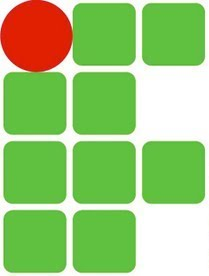
\includegraphics[width=0.8cm]{images/logo.jpg}}

\begin{document}
   \begin{frame}
      \titlepage
   \end{frame}

   \begin{frame}{\contentsname}
      \tableofcontents
   \end{frame}

   \section{Introdução}
   \begin{frame}{Introdução}
      \begin{itemize}
         \item<+-> Projeto CGT
         \item<+-> Vínculo CNPQ
         \item<+-> Ferramenta de criação de jogos
         \begin{itemize}
            \item<+-> Robusta
            \item<+-> Sem \emph{feedback}
            \item<+-> Controles confusos
            \item<+-> Processo de criação demorado
         \end{itemize}
      \end{itemize}
   \end{frame}

   \begin{frame}
      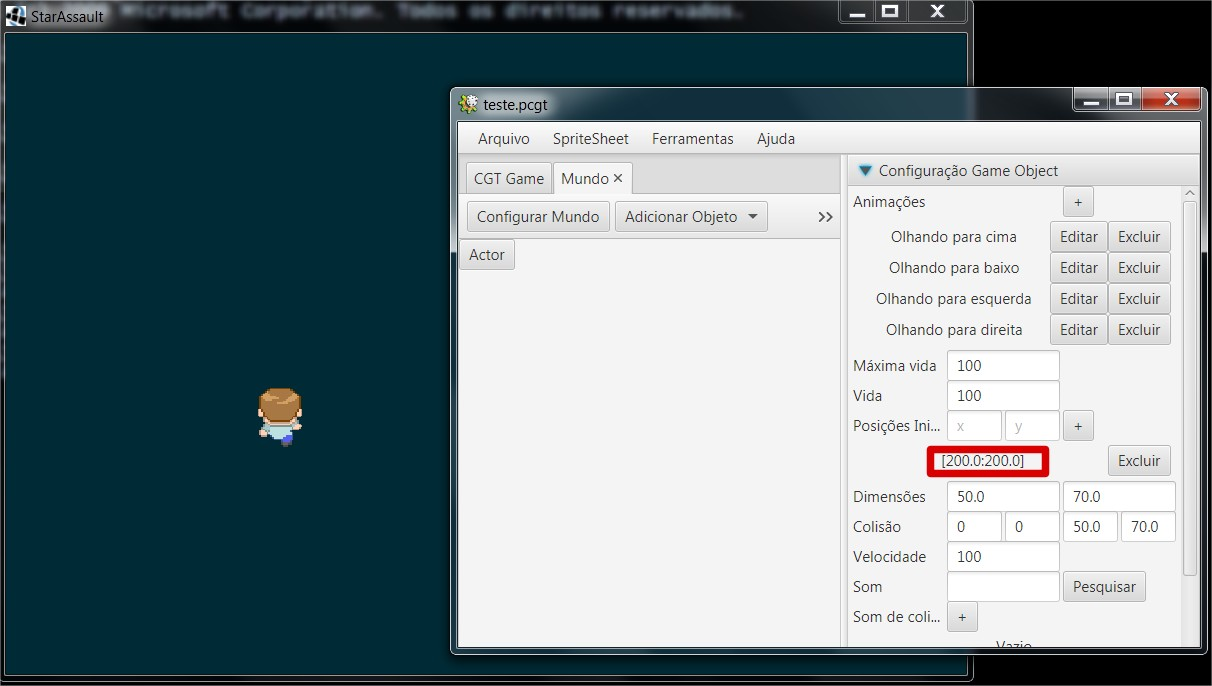
\includegraphics[width=\textwidth]{images/problema-1.jpg}
   \end{frame}

   \begin{frame}
      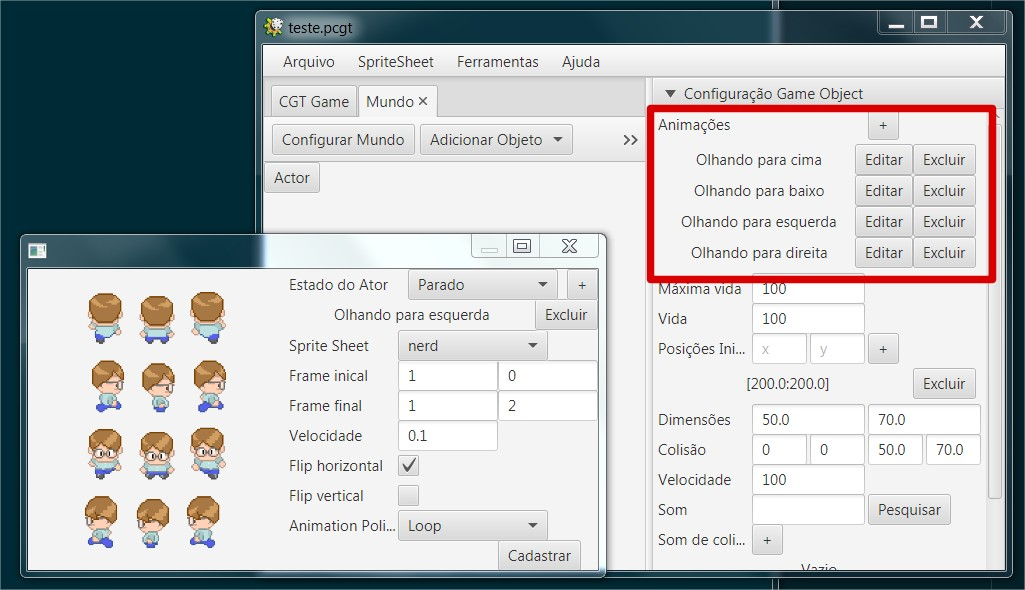
\includegraphics[width=\textwidth]{images/problema-2.jpg}
   \end{frame}

   \section{Problemas}
   \begin{frame}{Problema}
      \begin{block}{Organização dos objetos do jogo}
         \begin{itemize}
            \item<+-> Jogos longos
            \item<+-> Hierarquia
            \item<+-> As características importam
         \end{itemize}
      \end{block}
   \end{frame}

   \begin{frame}
      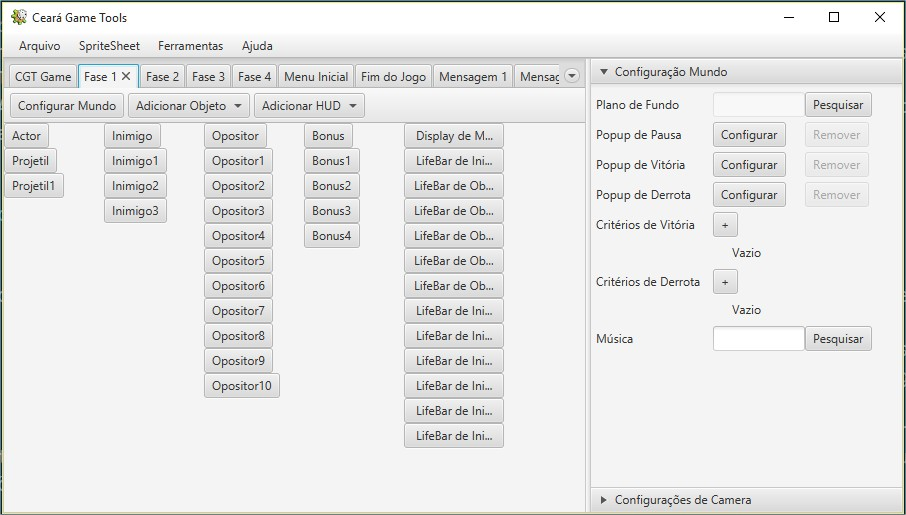
\includegraphics[width=\textwidth]{images/objetos_disposicao.jpg}
   \end{frame}

   \begin{frame}{Problema}
      \begin{block}{Painéis de configuração}
         \begin{itemize}
            \item<+-> Devem ser claros
            \item<+-> Significado de cada propriedade
         \end{itemize}
      \end{block}
   \end{frame}

   \begin{frame}
      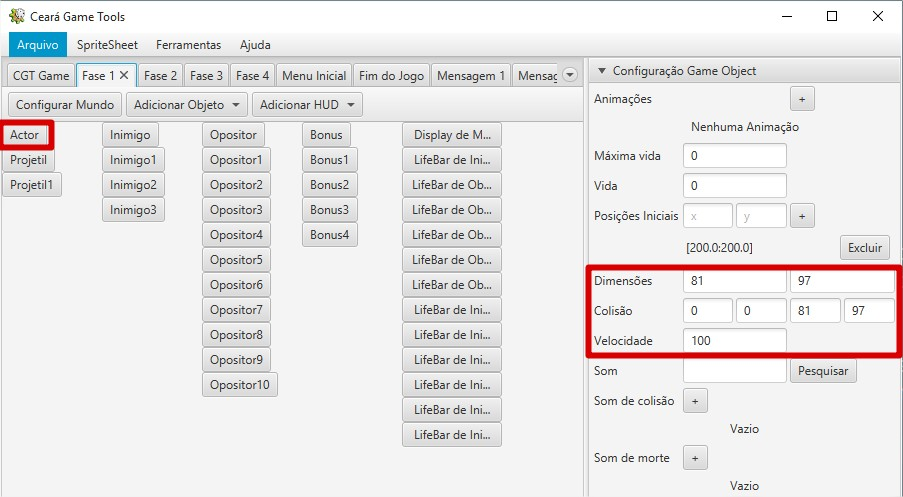
\includegraphics[width=\textwidth]{images/obj_dimensoes.jpg}
   \end{frame}

   \begin{frame}{Problema}
      \begin{block}{Pré visualização}
         \begin{itemize}
            \item<+-> Simulação do jogo
            \item<+-> Características que precisam
         \end{itemize}
      \end{block}
   \end{frame}

   \begin{frame}
      \begin{center}
         \begin{tabular}{p{12em} | p{12em}}
            \textbf{Objeto(s)} & \textbf{Atributo(s)} \\
            \hline
            Mundo e tela do jogo & Plano de fundo \\
            \hline
            Ator, inimigo, bônus, opositor e projétil & Animações (\emph{spritesheet}), posição inicial, dimensões e área de colisão. \\
            \hline
            Botão de uma tela & Posição, dimensões, textura do botão normal e textura quando for pressionado.\\
            \hline
            Munição do projétil & Posição, dimensões e ícone. \\
            \hline
            Barra de vida de um objeto & Posição, dimensões, textura do preenchimento da barra e textura do plano de fundo. \\
         \end{tabular}
      \end{center}
   \end{frame}

   \section{Melhorias}

   \section{Estudo de caso}

\end{document}
